\documentclass[twoside]{book}

% Packages required by doxygen
\usepackage{fixltx2e}
\usepackage{calc}
\usepackage{doxygen}
\usepackage[export]{adjustbox} % also loads graphicx
\usepackage{graphicx}
\usepackage[utf8]{inputenc}
\usepackage{makeidx}
\usepackage{multicol}
\usepackage{multirow}
\PassOptionsToPackage{warn}{textcomp}
\usepackage{textcomp}
\usepackage[nointegrals]{wasysym}
\usepackage[table]{xcolor}

% Font selection
\usepackage[T1]{fontenc}
\usepackage[scaled=.90]{helvet}
\usepackage{courier}
\usepackage{amssymb}
\usepackage{sectsty}
\renewcommand{\familydefault}{\sfdefault}
\allsectionsfont{%
  \fontseries{bc}\selectfont%
  \color{darkgray}%
}
\renewcommand{\DoxyLabelFont}{%
  \fontseries{bc}\selectfont%
  \color{darkgray}%
}
\newcommand{\+}{\discretionary{\mbox{\scriptsize$\hookleftarrow$}}{}{}}

% Page & text layout
\usepackage{geometry}
\geometry{%
  a4paper,%
  top=2.5cm,%
  bottom=2.5cm,%
  left=2.5cm,%
  right=2.5cm%
}
\tolerance=750
\hfuzz=15pt
\hbadness=750
\setlength{\emergencystretch}{15pt}
\setlength{\parindent}{0cm}
\setlength{\parskip}{3ex plus 2ex minus 2ex}
\makeatletter
\renewcommand{\paragraph}{%
  \@startsection{paragraph}{4}{0ex}{-1.0ex}{1.0ex}{%
    \normalfont\normalsize\bfseries\SS@parafont%
  }%
}
\renewcommand{\subparagraph}{%
  \@startsection{subparagraph}{5}{0ex}{-1.0ex}{1.0ex}{%
    \normalfont\normalsize\bfseries\SS@subparafont%
  }%
}
\makeatother

% Headers & footers
\usepackage{fancyhdr}
\pagestyle{fancyplain}
\fancyhead[LE]{\fancyplain{}{\bfseries\thepage}}
\fancyhead[CE]{\fancyplain{}{}}
\fancyhead[RE]{\fancyplain{}{\bfseries\leftmark}}
\fancyhead[LO]{\fancyplain{}{\bfseries\rightmark}}
\fancyhead[CO]{\fancyplain{}{}}
\fancyhead[RO]{\fancyplain{}{\bfseries\thepage}}
\fancyfoot[LE]{\fancyplain{}{}}
\fancyfoot[CE]{\fancyplain{}{}}
\fancyfoot[RE]{\fancyplain{}{\bfseries\scriptsize Generated by Doxygen }}
\fancyfoot[LO]{\fancyplain{}{\bfseries\scriptsize Generated by Doxygen }}
\fancyfoot[CO]{\fancyplain{}{}}
\fancyfoot[RO]{\fancyplain{}{}}
\renewcommand{\footrulewidth}{0.4pt}
\renewcommand{\chaptermark}[1]{%
  \markboth{#1}{}%
}
\renewcommand{\sectionmark}[1]{%
  \markright{\thesection\ #1}%
}

% Indices & bibliography
\usepackage{natbib}
\usepackage[titles]{tocloft}
\setcounter{tocdepth}{3}
\setcounter{secnumdepth}{5}
\makeindex

% Hyperlinks (required, but should be loaded last)
\usepackage{ifpdf}
\ifpdf
  \usepackage[pdftex,pagebackref=true]{hyperref}
\else
  \usepackage[ps2pdf,pagebackref=true]{hyperref}
\fi
\hypersetup{%
  colorlinks=true,%
  linkcolor=blue,%
  citecolor=blue,%
  unicode%
}

% Custom commands
\newcommand{\clearemptydoublepage}{%
  \newpage{\pagestyle{empty}\cleardoublepage}%
}

\usepackage{caption}
\captionsetup{labelsep=space,justification=centering,font={bf},singlelinecheck=off,skip=4pt,position=top}

%===== C O N T E N T S =====

\begin{document}

% Titlepage & ToC
\hypersetup{pageanchor=false,
             bookmarksnumbered=true,
             pdfencoding=unicode
            }
\pagenumbering{roman}
\begin{titlepage}
\vspace*{7cm}
\begin{center}%
{\Large Nano\+Mag\+View \\[1ex]\large v0.\+01 }\\
\vspace*{1cm}
{\large Generated by Doxygen 1.8.11}\\
\end{center}
\end{titlepage}
\clearemptydoublepage
\tableofcontents
\clearemptydoublepage
\pagenumbering{arabic}
\hypersetup{pageanchor=true}

%--- Begin generated contents ---
\chapter{Nano\+Mag\+View}
\label{index}\hypertarget{index}{}Simple Application to View Output Files from Nano\+Mag\+MC

\subsection*{Requirements}


\begin{DoxyItemize}
\item Qt (tested using 5.\+10.\+1)
\item Open\+GL libs
\item H\+D\+F5 libs
\end{DoxyItemize}

\subsection*{Installation}


\begin{DoxyItemize}
\item Clone the directory and \hyperlink{namespaceVFRendering}{V\+F\+Rendering} submodule using\+:
\end{DoxyItemize}

{\ttfamily git clone -\/-\/recursive \href{https://github.com/waterswims/NanoMagView.git}{\tt https\+://github.\+com/waterswims/\+Nano\+Mag\+View.\+git}}


\begin{DoxyItemize}
\item Generate the makefile using\+:
\end{DoxyItemize}

{\ttfamily qmake Nano\+Mag\+View.\+pro}


\begin{DoxyItemize}
\item Build the \hyperlink{namespaceVFRendering}{V\+F\+Rendering} library using\+:
\end{DoxyItemize}

{\ttfamily make build\+VF}


\begin{DoxyItemize}
\item Build the application using\+:
\end{DoxyItemize}

{\ttfamily make}

\subsection*{Acknowledgements}

This project used the \hyperlink{namespaceVFRendering}{V\+F\+Rendering} library which can be found at \href{https://github.com/spirit-code/VFRendering}{\tt https\+://github.\+com/spirit-\/code/\+V\+F\+Rendering} 
\chapter{Namespace Index}
\section{Namespace List}
Here is a list of all namespaces with brief descriptions\+:\begin{DoxyCompactList}
\item\contentsline{section}{\hyperlink{namespaceh5Input}{h5\+Input} }{\pageref{d3/df3/namespaceh5Input}}{}
\item\contentsline{section}{\hyperlink{namespacenMagWindows}{n\+Mag\+Windows} }{\pageref{d1/d3c/namespacenMagWindows}}{}
\item\contentsline{section}{\hyperlink{namespaceVFRendering}{V\+F\+Rendering} }{\pageref{d4/dbe/namespaceVFRendering}}{}
\end{DoxyCompactList}

\chapter{Hierarchical Index}
\section{Class Hierarchy}
This inheritance list is sorted roughly, but not completely, alphabetically\+:\begin{DoxyCompactList}
\item Q\+Object\begin{DoxyCompactList}
\item \contentsline{section}{n\+Mag\+Windows\+:\+:viewer\+Instance}{\pageref{classnMagWindows_1_1viewerInstance}}{}
\end{DoxyCompactList}
\item Q\+Open\+G\+L\+Widget\begin{DoxyCompactList}
\item \contentsline{section}{n\+Mag\+Windows\+:\+:viewer\+Window}{\pageref{classnMagWindows_1_1viewerWindow}}{}
\end{DoxyCompactList}
\item Q\+Widget\begin{DoxyCompactList}
\item \contentsline{section}{n\+Mag\+Windows\+:\+:render\+Options\+Window}{\pageref{classnMagWindows_1_1renderOptionsWindow}}{}
\item \contentsline{section}{n\+Mag\+Windows\+:\+:select\+T\+H\+Window}{\pageref{classnMagWindows_1_1selectTHWindow}}{}
\end{DoxyCompactList}
\end{DoxyCompactList}

\chapter{Class Index}
\section{Class List}
Here are the classes, structs, unions and interfaces with brief descriptions\+:\begin{DoxyCompactList}
\item\contentsline{section}{\hyperlink{classnMagWindows_1_1renderOptionsWindow}{n\+Mag\+Windows\+::render\+Options\+Window} }{\pageref{d0/d13/classnMagWindows_1_1renderOptionsWindow}}{}
\item\contentsline{section}{\hyperlink{classnMagWindows_1_1selectTHWindow}{n\+Mag\+Windows\+::select\+T\+H\+Window} }{\pageref{d0/dea/classnMagWindows_1_1selectTHWindow}}{}
\item\contentsline{section}{\hyperlink{classnMagWindows_1_1viewerInstance}{n\+Mag\+Windows\+::viewer\+Instance} }{\pageref{dd/d14/classnMagWindows_1_1viewerInstance}}{}
\item\contentsline{section}{\hyperlink{classnMagWindows_1_1viewerWindow}{n\+Mag\+Windows\+::viewer\+Window} }{\pageref{db/d64/classnMagWindows_1_1viewerWindow}}{}
\end{DoxyCompactList}

\chapter{File Index}
\section{File List}
Here is a list of all files with brief descriptions\+:\begin{DoxyCompactList}
\item\contentsline{section}{include/\hyperlink{array__alloc_8hpp}{array\+\_\+alloc.\+hpp} }{\pageref{dc/df8/array__alloc_8hpp}}{}
\item\contentsline{section}{include/\hyperlink{h5Input_8hpp}{h5\+Input.\+hpp} }{\pageref{d5/d22/h5Input_8hpp}}{}
\item\contentsline{section}{include/\hyperlink{renderOptions_8hpp}{render\+Options.\+hpp} }{\pageref{df/d8e/renderOptions_8hpp}}{}
\item\contentsline{section}{include/\hyperlink{selectLatt_8hpp}{select\+Latt.\+hpp} }{\pageref{d9/d33/selectLatt_8hpp}}{}
\item\contentsline{section}{include/\hyperlink{viewerInstance_8hpp}{viewer\+Instance.\+hpp} }{\pageref{da/da9/viewerInstance_8hpp}}{}
\item\contentsline{section}{include/\hyperlink{viewerWindow_8hpp}{viewer\+Window.\+hpp} }{\pageref{dc/d67/viewerWindow_8hpp}}{}
\end{DoxyCompactList}

\chapter{Namespace Documentation}
\hypertarget{namespaceh5Input}{}\section{h5\+Input Namespace Reference}
\label{namespaceh5Input}\index{h5\+Input@{h5\+Input}}
\subsection*{Functions}
\begin{DoxyCompactItemize}
\item 
void \hyperlink{namespaceh5Input_a7e2655a571daa8f456bc2a22eec1ef3d}{get\+Field\+Temps} (std\+::string file\+Name, std\+::vector$<$ float $>$ \&Ts, std\+::vector$<$ float $>$ \&Hs)
\item 
void \hyperlink{namespaceh5Input_a4894a89d7f105d15e01f6c270d45b47a}{get\+Spins} (std\+::string file\+Name, const int Tind, const int Hind, V\+F\+Rendering\+::\+Geometry \&geometry, std\+::vector$<$ glm\+::vec3 $>$ \&directions, std\+::vector$<$ double $>$ \&z\+\_\+pos)
\end{DoxyCompactItemize}


\subsection{Function Documentation}
\index{h5\+Input@{h5\+Input}!get\+Field\+Temps@{get\+Field\+Temps}}
\index{get\+Field\+Temps@{get\+Field\+Temps}!h5\+Input@{h5\+Input}}
\subsubsection[{\texorpdfstring{get\+Field\+Temps(std\+::string file\+Name, std\+::vector$<$ float $>$ \&\+Ts, std\+::vector$<$ float $>$ \&\+Hs)}{getFieldTemps(std::string fileName, std::vector< float > &Ts, std::vector< float > &Hs)}}]{\setlength{\rightskip}{0pt plus 5cm}void h5\+Input\+::get\+Field\+Temps (
\begin{DoxyParamCaption}
\item[{std\+::string}]{file\+Name, }
\item[{std\+::vector$<$ float $>$ \&}]{Ts, }
\item[{std\+::vector$<$ float $>$ \&}]{Hs}
\end{DoxyParamCaption}
)}\hypertarget{namespaceh5Input_a7e2655a571daa8f456bc2a22eec1ef3d}{}\label{namespaceh5Input_a7e2655a571daa8f456bc2a22eec1ef3d}
Function which extracts the fields and temperatures for which lattices exist in a specified H\+D\+F5 file.

/param file\+Name The name of the input H\+D\+F5 file /param Ts A vector of floats where the temperatures will be placed /param Hs A vector of floats where the fields will be placed \index{h5\+Input@{h5\+Input}!get\+Spins@{get\+Spins}}
\index{get\+Spins@{get\+Spins}!h5\+Input@{h5\+Input}}
\subsubsection[{\texorpdfstring{get\+Spins(std\+::string file\+Name, const int Tind, const int Hind, V\+F\+Rendering\+::\+Geometry \&geometry, std\+::vector$<$ glm\+::vec3 $>$ \&directions, std\+::vector$<$ double $>$ \&z\+\_\+pos)}{getSpins(std::string fileName, const int Tind, const int Hind, VFRendering::Geometry &geometry, std::vector< glm::vec3 > &directions, std::vector< double > &z_pos)}}]{\setlength{\rightskip}{0pt plus 5cm}void h5\+Input\+::get\+Spins (
\begin{DoxyParamCaption}
\item[{std\+::string}]{file\+Name, }
\item[{const int}]{Tind, }
\item[{const int}]{Hind, }
\item[{V\+F\+Rendering\+::\+Geometry \&}]{geometry, }
\item[{std\+::vector$<$ glm\+::vec3 $>$ \&}]{directions, }
\item[{std\+::vector$<$ double $>$ \&}]{z\+\_\+pos}
\end{DoxyParamCaption}
)}\hypertarget{namespaceh5Input_a4894a89d7f105d15e01f6c270d45b47a}{}\label{namespaceh5Input_a4894a89d7f105d15e01f6c270d45b47a}
Function which extracts the spin values at a specific field and temperature

/param file\+Name The name of the input H\+D\+F5 file /param Tind The index of the chosen temperature /param Hind The index of the chosen field /param geometry The geometry of the lattice /param directions The directions of the spins 
\hypertarget{namespacenMagWindows}{}\section{n\+Mag\+Windows Namespace Reference}
\label{namespacenMagWindows}\index{n\+Mag\+Windows@{n\+Mag\+Windows}}
\subsection*{Classes}
\begin{DoxyCompactItemize}
\item 
class \hyperlink{classnMagWindows_1_1renderOptionsWindow}{render\+Options\+Window}
\item 
class \hyperlink{classnMagWindows_1_1selectTHWindow}{select\+T\+H\+Window}
\item 
class \hyperlink{classnMagWindows_1_1viewerInstance}{viewer\+Instance}
\item 
class \hyperlink{classnMagWindows_1_1viewerWindow}{viewer\+Window}
\end{DoxyCompactItemize}

\hypertarget{namespaceVFRendering}{}\section{V\+F\+Rendering Namespace Reference}
\label{namespaceVFRendering}\index{V\+F\+Rendering@{V\+F\+Rendering}}

\chapter{Class Documentation}
\hypertarget{classnMagWindows_1_1renderOptionsWindow}{}\section{n\+Mag\+Windows\+:\+:render\+Options\+Window Class Reference}
\label{classnMagWindows_1_1renderOptionsWindow}\index{n\+Mag\+Windows\+::render\+Options\+Window@{n\+Mag\+Windows\+::render\+Options\+Window}}


{\ttfamily \#include $<$render\+Options.\+hpp$>$}



Inheritance diagram for n\+Mag\+Windows\+:\+:render\+Options\+Window\+:
\nopagebreak
\begin{figure}[H]
\begin{center}
\leavevmode
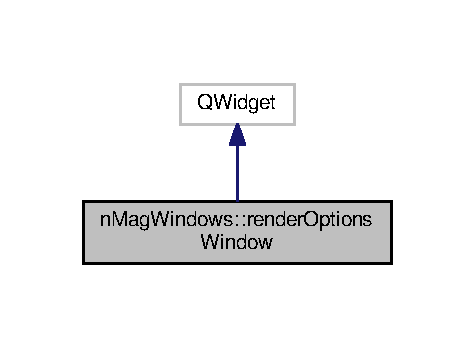
\includegraphics[width=228pt]{d1/d6c/classnMagWindows_1_1renderOptionsWindow__inherit__graph}
\end{center}
\end{figure}


Collaboration diagram for n\+Mag\+Windows\+:\+:render\+Options\+Window\+:
\nopagebreak
\begin{figure}[H]
\begin{center}
\leavevmode
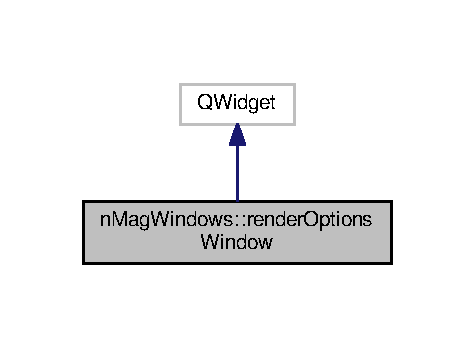
\includegraphics[width=228pt]{d4/da3/classnMagWindows_1_1renderOptionsWindow__coll__graph}
\end{center}
\end{figure}
\subsection*{Signals}
\begin{DoxyCompactItemize}
\item 
void \hyperlink{classnMagWindows_1_1renderOptionsWindow_a3f4c6255201e8fd5f4eacda97b58a5e2}{send\+Update} (bool arr\+On, bool all\+On, std\+::vector$<$ int $>$ slices, bool iso\+On, double iso\+Val)
\end{DoxyCompactItemize}
\subsection*{Public Member Functions}
\begin{DoxyCompactItemize}
\item 
\hyperlink{classnMagWindows_1_1renderOptionsWindow_a9ff82b1f7651b20407c42df97e898f19}{render\+Options\+Window} ()
\begin{DoxyCompactList}\small\item\em Constructor. \end{DoxyCompactList}\end{DoxyCompactItemize}


\subsection{Constructor \& Destructor Documentation}
\index{n\+Mag\+Windows\+::render\+Options\+Window@{n\+Mag\+Windows\+::render\+Options\+Window}!render\+Options\+Window@{render\+Options\+Window}}
\index{render\+Options\+Window@{render\+Options\+Window}!n\+Mag\+Windows\+::render\+Options\+Window@{n\+Mag\+Windows\+::render\+Options\+Window}}
\subsubsection[{\texorpdfstring{render\+Options\+Window()}{renderOptionsWindow()}}]{\setlength{\rightskip}{0pt plus 5cm}n\+Mag\+Windows\+::render\+Options\+Window\+::render\+Options\+Window (
\begin{DoxyParamCaption}
{}
\end{DoxyParamCaption}
)}\hypertarget{classnMagWindows_1_1renderOptionsWindow_a9ff82b1f7651b20407c42df97e898f19}{}\label{classnMagWindows_1_1renderOptionsWindow_a9ff82b1f7651b20407c42df97e898f19}


Constructor. 



\subsection{Member Function Documentation}
\index{n\+Mag\+Windows\+::render\+Options\+Window@{n\+Mag\+Windows\+::render\+Options\+Window}!send\+Update@{send\+Update}}
\index{send\+Update@{send\+Update}!n\+Mag\+Windows\+::render\+Options\+Window@{n\+Mag\+Windows\+::render\+Options\+Window}}
\subsubsection[{\texorpdfstring{send\+Update}{sendUpdate}}]{\setlength{\rightskip}{0pt plus 5cm}void n\+Mag\+Windows\+::render\+Options\+Window\+::send\+Update (
\begin{DoxyParamCaption}
\item[{bool}]{arr\+On, }
\item[{bool}]{all\+On, }
\item[{std\+::vector$<$ int $>$}]{slices, }
\item[{bool}]{iso\+On, }
\item[{double}]{iso\+Val}
\end{DoxyParamCaption}
)\hspace{0.3cm}{\ttfamily [signal]}}\hypertarget{classnMagWindows_1_1renderOptionsWindow_a3f4c6255201e8fd5f4eacda97b58a5e2}{}\label{classnMagWindows_1_1renderOptionsWindow_a3f4c6255201e8fd5f4eacda97b58a5e2}
Sends the chosen slices and iso value

/param arr\+On Arrow switch /param all\+On Turn on all arrows /param slices Slices for the arrow /param iso\+On Isosurface switch /param iso\+Val Value at which isosurface is drawn 

The documentation for this class was generated from the following file\+:\begin{DoxyCompactItemize}
\item 
include/\hyperlink{renderOptions_8hpp}{render\+Options.\+hpp}\end{DoxyCompactItemize}

\hypertarget{classnMagWindows_1_1selectTHWindow}{}\section{n\+Mag\+Windows\+:\+:select\+T\+H\+Window Class Reference}
\label{classnMagWindows_1_1selectTHWindow}\index{n\+Mag\+Windows\+::select\+T\+H\+Window@{n\+Mag\+Windows\+::select\+T\+H\+Window}}


{\ttfamily \#include $<$select\+Latt.\+hpp$>$}



Inheritance diagram for n\+Mag\+Windows\+:\+:select\+T\+H\+Window\+:\nopagebreak
\begin{figure}[H]
\begin{center}
\leavevmode
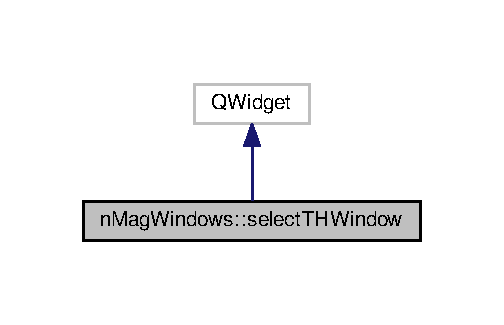
\includegraphics[width=242pt]{d7/dd6/classnMagWindows_1_1selectTHWindow__inherit__graph}
\end{center}
\end{figure}


Collaboration diagram for n\+Mag\+Windows\+:\+:select\+T\+H\+Window\+:\nopagebreak
\begin{figure}[H]
\begin{center}
\leavevmode
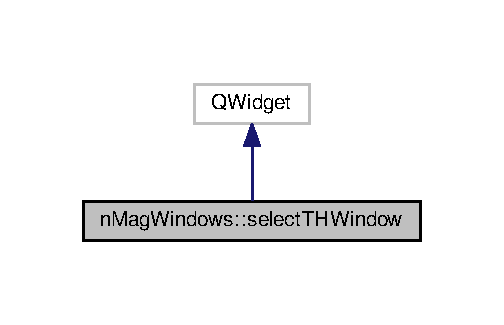
\includegraphics[width=242pt]{df/df2/classnMagWindows_1_1selectTHWindow__coll__graph}
\end{center}
\end{figure}
\subsection*{Public Member Functions}
\begin{DoxyCompactItemize}
\item 
\hyperlink{classnMagWindows_1_1selectTHWindow_a57ec8a7a07a4b37031738674cb3bdb85}{select\+T\+H\+Window} (std\+::string h5\+Name\+In)
\end{DoxyCompactItemize}


\subsection{Constructor \& Destructor Documentation}
\index{n\+Mag\+Windows\+::select\+T\+H\+Window@{n\+Mag\+Windows\+::select\+T\+H\+Window}!select\+T\+H\+Window@{select\+T\+H\+Window}}
\index{select\+T\+H\+Window@{select\+T\+H\+Window}!n\+Mag\+Windows\+::select\+T\+H\+Window@{n\+Mag\+Windows\+::select\+T\+H\+Window}}
\subsubsection[{\texorpdfstring{select\+T\+H\+Window(std\+::string h5\+Name\+In)}{selectTHWindow(std::string h5NameIn)}}]{\setlength{\rightskip}{0pt plus 5cm}n\+Mag\+Windows\+::select\+T\+H\+Window\+::select\+T\+H\+Window (
\begin{DoxyParamCaption}
\item[{std\+::string}]{h5\+Name\+In}
\end{DoxyParamCaption}
)}\hypertarget{classnMagWindows_1_1selectTHWindow_a57ec8a7a07a4b37031738674cb3bdb85}{}\label{classnMagWindows_1_1selectTHWindow_a57ec8a7a07a4b37031738674cb3bdb85}
Constructor


\begin{DoxyParams}{Parameters}
{\em h5\+Name\+In} & The name of the chosen H\+D\+F5 file \\
\hline
\end{DoxyParams}


The documentation for this class was generated from the following file\+:\begin{DoxyCompactItemize}
\item 
include/\hyperlink{selectLatt_8hpp}{select\+Latt.\+hpp}\end{DoxyCompactItemize}

\hypertarget{classnMagWindows_1_1viewerInstance}{}\section{n\+Mag\+Windows\+:\+:viewer\+Instance Class Reference}
\label{classnMagWindows_1_1viewerInstance}\index{n\+Mag\+Windows\+::viewer\+Instance@{n\+Mag\+Windows\+::viewer\+Instance}}


{\ttfamily \#include $<$viewer\+Instance.\+hpp$>$}



Inheritance diagram for n\+Mag\+Windows\+:\+:viewer\+Instance\+:\nopagebreak
\begin{figure}[H]
\begin{center}
\leavevmode
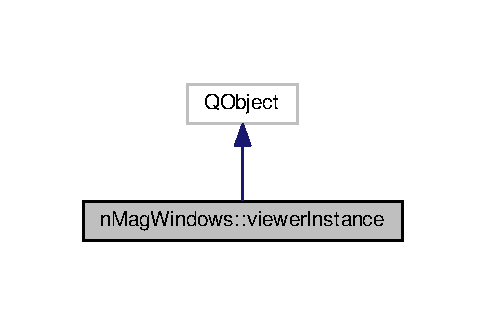
\includegraphics[width=233pt]{d6/d37/classnMagWindows_1_1viewerInstance__inherit__graph}
\end{center}
\end{figure}


Collaboration diagram for n\+Mag\+Windows\+:\+:viewer\+Instance\+:\nopagebreak
\begin{figure}[H]
\begin{center}
\leavevmode
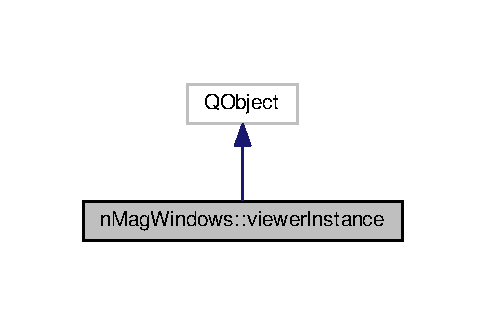
\includegraphics[width=233pt]{d1/d85/classnMagWindows_1_1viewerInstance__coll__graph}
\end{center}
\end{figure}
\subsection*{Public Member Functions}
\begin{DoxyCompactItemize}
\item 
\hyperlink{classnMagWindows_1_1viewerInstance_ad6cc22c4ff86766ab0cae5986164391b}{viewer\+Instance} (std\+::string h5\+Name, int T\+Ind, int H\+Ind, Q\+Object $\ast$parent=Q\+\_\+\+N\+U\+L\+L\+P\+TR)
\end{DoxyCompactItemize}


\subsection{Constructor \& Destructor Documentation}
\index{n\+Mag\+Windows\+::viewer\+Instance@{n\+Mag\+Windows\+::viewer\+Instance}!viewer\+Instance@{viewer\+Instance}}
\index{viewer\+Instance@{viewer\+Instance}!n\+Mag\+Windows\+::viewer\+Instance@{n\+Mag\+Windows\+::viewer\+Instance}}
\subsubsection[{\texorpdfstring{viewer\+Instance(std\+::string h5\+Name, int T\+Ind, int H\+Ind, Q\+Object $\ast$parent=\+Q\+\_\+\+N\+U\+L\+L\+P\+T\+R)}{viewerInstance(std::string h5Name, int TInd, int HInd, QObject *parent=Q_NULLPTR)}}]{\setlength{\rightskip}{0pt plus 5cm}n\+Mag\+Windows\+::viewer\+Instance\+::viewer\+Instance (
\begin{DoxyParamCaption}
\item[{std\+::string}]{h5\+Name, }
\item[{int}]{T\+Ind, }
\item[{int}]{H\+Ind, }
\item[{Q\+Object $\ast$}]{parent = {\ttfamily Q\+\_\+NULLPTR}}
\end{DoxyParamCaption}
)}\hypertarget{classnMagWindows_1_1viewerInstance_ad6cc22c4ff86766ab0cae5986164391b}{}\label{classnMagWindows_1_1viewerInstance_ad6cc22c4ff86766ab0cae5986164391b}
Constructor


\begin{DoxyParams}{Parameters}
{\em h5\+Name\+In} & The name of the chosen H\+D\+F5 file \\
\hline
{\em T\+Ind} & The index of the chosen temperature. \\
\hline
{\em H\+Ind} & The index of the chosen field. \\
\hline
{\em parent} & The parent QT object. \\
\hline
\end{DoxyParams}


The documentation for this class was generated from the following file\+:\begin{DoxyCompactItemize}
\item 
include/\hyperlink{viewerInstance_8hpp}{viewer\+Instance.\+hpp}\end{DoxyCompactItemize}

\hypertarget{classnMagWindows_1_1viewerWindow}{}\section{n\+Mag\+Windows\+:\+:viewer\+Window Class Reference}
\label{classnMagWindows_1_1viewerWindow}\index{n\+Mag\+Windows\+::viewer\+Window@{n\+Mag\+Windows\+::viewer\+Window}}


{\ttfamily \#include $<$viewer\+Window.\+hpp$>$}



Inheritance diagram for n\+Mag\+Windows\+:\+:viewer\+Window\+:
\nopagebreak
\begin{figure}[H]
\begin{center}
\leavevmode
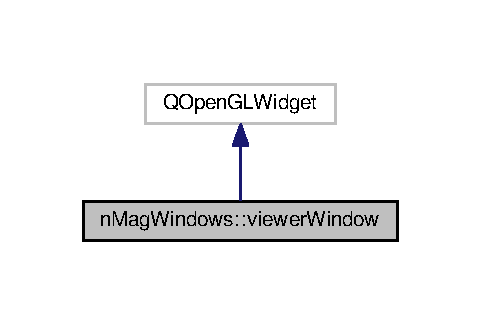
\includegraphics[width=231pt]{d0/d95/classnMagWindows_1_1viewerWindow__inherit__graph}
\end{center}
\end{figure}


Collaboration diagram for n\+Mag\+Windows\+:\+:viewer\+Window\+:
\nopagebreak
\begin{figure}[H]
\begin{center}
\leavevmode
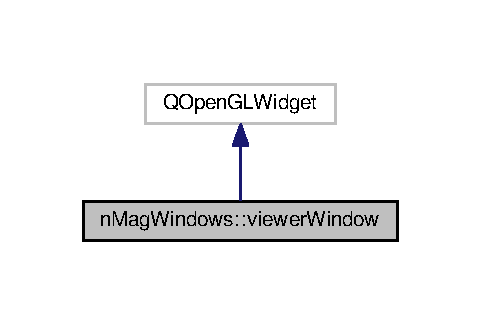
\includegraphics[width=231pt]{d8/d51/classnMagWindows_1_1viewerWindow__coll__graph}
\end{center}
\end{figure}
\subsection*{Public Member Functions}
\begin{DoxyCompactItemize}
\item 
\hyperlink{classnMagWindows_1_1viewerWindow_a700e4bca76465101c5404ed3511af38f}{viewer\+Window} (std\+::vector$<$ double $>$ slice\+\_\+pos\+\_\+in, const bool arrow\+On, const bool all\+Arrow, const std\+::vector$<$ int $>$ slices, const bool iso\+On, const double iso\+Val, Q\+Widget $\ast$parent=nullptr)
\item 
virtual \hyperlink{classnMagWindows_1_1viewerWindow_abc66dbe51c1fd662eafcb14466382655}{$\sim$viewer\+Window} ()
\item 
void \hyperlink{classnMagWindows_1_1viewerWindow_a91e38c0e40f40aa4219c7b9bccfdca21}{update} (const V\+F\+Rendering\+::\+Geometry \&geometry, const std\+::vector$<$ glm\+::vec3 $>$ \&vectors)
\item 
void \hyperlink{classnMagWindows_1_1viewerWindow_aa93ecd1a2bc515804cc5780902111206}{update\+Vectors} (const std\+::vector$<$ glm\+::vec3 $>$ \&vectors)
\item 
void \hyperlink{classnMagWindows_1_1viewerWindow_ad3c57658a50c31f5680ca0149f4ed700}{update\+Options} (const V\+F\+Rendering\+::\+Options \&options)
\item 
void \hyperlink{classnMagWindows_1_1viewerWindow_a9336f6f66088169a5a4ce979755427ba}{set\+\_\+renderers} (const bool arrow\+On, const bool all\+Arrow, const std\+::vector$<$ int $>$ slices, const bool iso\+On, const double iso\+Val)
\item 
float \hyperlink{classnMagWindows_1_1viewerWindow_a8d1bdb9fd44982e2f82716a70bc5fb05}{get\+Framerate} () const 
\end{DoxyCompactItemize}
\subsection*{Protected Member Functions}
\begin{DoxyCompactItemize}
\item 
void \hyperlink{classnMagWindows_1_1viewerWindow_a38e32a190bcd85e1a78fbf13c2e5bf2f}{initialize\+GL} () override
\item 
void \hyperlink{classnMagWindows_1_1viewerWindow_affcbcf6e86f76f64d4492372ebcc0aca}{resize\+GL} (int width, int height) override
\item 
void \hyperlink{classnMagWindows_1_1viewerWindow_a4dc51c39e4bb00f9622efb4a2683ce94}{paint\+GL} () override
\item 
void \hyperlink{classnMagWindows_1_1viewerWindow_a5ec1c19ffa3287dfece38f7db63c80ec}{wheel\+Event} (Q\+Wheel\+Event $\ast$event) override
\item 
void \hyperlink{classnMagWindows_1_1viewerWindow_ab10703ac3a707a6b813862255b606b51}{mouse\+Press\+Event} (Q\+Mouse\+Event $\ast$event) override
\item 
void \hyperlink{classnMagWindows_1_1viewerWindow_ae844f52b23024f772a8175aa1fa395d7}{mouse\+Move\+Event} (Q\+Mouse\+Event $\ast$event) override
\end{DoxyCompactItemize}


\subsection{Constructor \& Destructor Documentation}
\index{n\+Mag\+Windows\+::viewer\+Window@{n\+Mag\+Windows\+::viewer\+Window}!viewer\+Window@{viewer\+Window}}
\index{viewer\+Window@{viewer\+Window}!n\+Mag\+Windows\+::viewer\+Window@{n\+Mag\+Windows\+::viewer\+Window}}
\subsubsection[{\texorpdfstring{viewer\+Window(std\+::vector$<$ double $>$ slice\+\_\+pos\+\_\+in, const bool arrow\+On, const bool all\+Arrow, const std\+::vector$<$ int $>$ slices, const bool iso\+On, const double iso\+Val, Q\+Widget $\ast$parent=nullptr)}{viewerWindow(std::vector< double > slice_pos_in, const bool arrowOn, const bool allArrow, const std::vector< int > slices, const bool isoOn, const double isoVal, QWidget *parent=nullptr)}}]{\setlength{\rightskip}{0pt plus 5cm}n\+Mag\+Windows\+::viewer\+Window\+::viewer\+Window (
\begin{DoxyParamCaption}
\item[{std\+::vector$<$ double $>$}]{slice\+\_\+pos\+\_\+in, }
\item[{const bool}]{arrow\+On, }
\item[{const bool}]{all\+Arrow, }
\item[{const std\+::vector$<$ int $>$}]{slices, }
\item[{const bool}]{iso\+On, }
\item[{const double}]{iso\+Val, }
\item[{Q\+Widget $\ast$}]{parent = {\ttfamily nullptr}}
\end{DoxyParamCaption}
)}\hypertarget{classnMagWindows_1_1viewerWindow_a700e4bca76465101c5404ed3511af38f}{}\label{classnMagWindows_1_1viewerWindow_a700e4bca76465101c5404ed3511af38f}
\index{n\+Mag\+Windows\+::viewer\+Window@{n\+Mag\+Windows\+::viewer\+Window}!````~viewer\+Window@{$\sim$viewer\+Window}}
\index{````~viewer\+Window@{$\sim$viewer\+Window}!n\+Mag\+Windows\+::viewer\+Window@{n\+Mag\+Windows\+::viewer\+Window}}
\subsubsection[{\texorpdfstring{$\sim$viewer\+Window()}{~viewerWindow()}}]{\setlength{\rightskip}{0pt plus 5cm}virtual n\+Mag\+Windows\+::viewer\+Window\+::$\sim$viewer\+Window (
\begin{DoxyParamCaption}
{}
\end{DoxyParamCaption}
)\hspace{0.3cm}{\ttfamily [virtual]}}\hypertarget{classnMagWindows_1_1viewerWindow_abc66dbe51c1fd662eafcb14466382655}{}\label{classnMagWindows_1_1viewerWindow_abc66dbe51c1fd662eafcb14466382655}


\subsection{Member Function Documentation}
\index{n\+Mag\+Windows\+::viewer\+Window@{n\+Mag\+Windows\+::viewer\+Window}!get\+Framerate@{get\+Framerate}}
\index{get\+Framerate@{get\+Framerate}!n\+Mag\+Windows\+::viewer\+Window@{n\+Mag\+Windows\+::viewer\+Window}}
\subsubsection[{\texorpdfstring{get\+Framerate() const }{getFramerate() const }}]{\setlength{\rightskip}{0pt plus 5cm}float n\+Mag\+Windows\+::viewer\+Window\+::get\+Framerate (
\begin{DoxyParamCaption}
{}
\end{DoxyParamCaption}
) const}\hypertarget{classnMagWindows_1_1viewerWindow_a8d1bdb9fd44982e2f82716a70bc5fb05}{}\label{classnMagWindows_1_1viewerWindow_a8d1bdb9fd44982e2f82716a70bc5fb05}
\index{n\+Mag\+Windows\+::viewer\+Window@{n\+Mag\+Windows\+::viewer\+Window}!initialize\+GL@{initialize\+GL}}
\index{initialize\+GL@{initialize\+GL}!n\+Mag\+Windows\+::viewer\+Window@{n\+Mag\+Windows\+::viewer\+Window}}
\subsubsection[{\texorpdfstring{initialize\+G\+L() override}{initializeGL() override}}]{\setlength{\rightskip}{0pt plus 5cm}void n\+Mag\+Windows\+::viewer\+Window\+::initialize\+GL (
\begin{DoxyParamCaption}
{}
\end{DoxyParamCaption}
)\hspace{0.3cm}{\ttfamily [override]}, {\ttfamily [protected]}}\hypertarget{classnMagWindows_1_1viewerWindow_a38e32a190bcd85e1a78fbf13c2e5bf2f}{}\label{classnMagWindows_1_1viewerWindow_a38e32a190bcd85e1a78fbf13c2e5bf2f}
\index{n\+Mag\+Windows\+::viewer\+Window@{n\+Mag\+Windows\+::viewer\+Window}!mouse\+Move\+Event@{mouse\+Move\+Event}}
\index{mouse\+Move\+Event@{mouse\+Move\+Event}!n\+Mag\+Windows\+::viewer\+Window@{n\+Mag\+Windows\+::viewer\+Window}}
\subsubsection[{\texorpdfstring{mouse\+Move\+Event(\+Q\+Mouse\+Event $\ast$event) override}{mouseMoveEvent(QMouseEvent *event) override}}]{\setlength{\rightskip}{0pt plus 5cm}void n\+Mag\+Windows\+::viewer\+Window\+::mouse\+Move\+Event (
\begin{DoxyParamCaption}
\item[{Q\+Mouse\+Event $\ast$}]{event}
\end{DoxyParamCaption}
)\hspace{0.3cm}{\ttfamily [override]}, {\ttfamily [protected]}}\hypertarget{classnMagWindows_1_1viewerWindow_ae844f52b23024f772a8175aa1fa395d7}{}\label{classnMagWindows_1_1viewerWindow_ae844f52b23024f772a8175aa1fa395d7}
\index{n\+Mag\+Windows\+::viewer\+Window@{n\+Mag\+Windows\+::viewer\+Window}!mouse\+Press\+Event@{mouse\+Press\+Event}}
\index{mouse\+Press\+Event@{mouse\+Press\+Event}!n\+Mag\+Windows\+::viewer\+Window@{n\+Mag\+Windows\+::viewer\+Window}}
\subsubsection[{\texorpdfstring{mouse\+Press\+Event(\+Q\+Mouse\+Event $\ast$event) override}{mousePressEvent(QMouseEvent *event) override}}]{\setlength{\rightskip}{0pt plus 5cm}void n\+Mag\+Windows\+::viewer\+Window\+::mouse\+Press\+Event (
\begin{DoxyParamCaption}
\item[{Q\+Mouse\+Event $\ast$}]{event}
\end{DoxyParamCaption}
)\hspace{0.3cm}{\ttfamily [override]}, {\ttfamily [protected]}}\hypertarget{classnMagWindows_1_1viewerWindow_ab10703ac3a707a6b813862255b606b51}{}\label{classnMagWindows_1_1viewerWindow_ab10703ac3a707a6b813862255b606b51}
\index{n\+Mag\+Windows\+::viewer\+Window@{n\+Mag\+Windows\+::viewer\+Window}!paint\+GL@{paint\+GL}}
\index{paint\+GL@{paint\+GL}!n\+Mag\+Windows\+::viewer\+Window@{n\+Mag\+Windows\+::viewer\+Window}}
\subsubsection[{\texorpdfstring{paint\+G\+L() override}{paintGL() override}}]{\setlength{\rightskip}{0pt plus 5cm}void n\+Mag\+Windows\+::viewer\+Window\+::paint\+GL (
\begin{DoxyParamCaption}
{}
\end{DoxyParamCaption}
)\hspace{0.3cm}{\ttfamily [override]}, {\ttfamily [protected]}}\hypertarget{classnMagWindows_1_1viewerWindow_a4dc51c39e4bb00f9622efb4a2683ce94}{}\label{classnMagWindows_1_1viewerWindow_a4dc51c39e4bb00f9622efb4a2683ce94}
\index{n\+Mag\+Windows\+::viewer\+Window@{n\+Mag\+Windows\+::viewer\+Window}!resize\+GL@{resize\+GL}}
\index{resize\+GL@{resize\+GL}!n\+Mag\+Windows\+::viewer\+Window@{n\+Mag\+Windows\+::viewer\+Window}}
\subsubsection[{\texorpdfstring{resize\+G\+L(int width, int height) override}{resizeGL(int width, int height) override}}]{\setlength{\rightskip}{0pt plus 5cm}void n\+Mag\+Windows\+::viewer\+Window\+::resize\+GL (
\begin{DoxyParamCaption}
\item[{int}]{width, }
\item[{int}]{height}
\end{DoxyParamCaption}
)\hspace{0.3cm}{\ttfamily [override]}, {\ttfamily [protected]}}\hypertarget{classnMagWindows_1_1viewerWindow_affcbcf6e86f76f64d4492372ebcc0aca}{}\label{classnMagWindows_1_1viewerWindow_affcbcf6e86f76f64d4492372ebcc0aca}
\index{n\+Mag\+Windows\+::viewer\+Window@{n\+Mag\+Windows\+::viewer\+Window}!set\+\_\+renderers@{set\+\_\+renderers}}
\index{set\+\_\+renderers@{set\+\_\+renderers}!n\+Mag\+Windows\+::viewer\+Window@{n\+Mag\+Windows\+::viewer\+Window}}
\subsubsection[{\texorpdfstring{set\+\_\+renderers(const bool arrow\+On, const bool all\+Arrow, const std\+::vector$<$ int $>$ slices, const bool iso\+On, const double iso\+Val)}{set_renderers(const bool arrowOn, const bool allArrow, const std::vector< int > slices, const bool isoOn, const double isoVal)}}]{\setlength{\rightskip}{0pt plus 5cm}void n\+Mag\+Windows\+::viewer\+Window\+::set\+\_\+renderers (
\begin{DoxyParamCaption}
\item[{const bool}]{arrow\+On, }
\item[{const bool}]{all\+Arrow, }
\item[{const std\+::vector$<$ int $>$}]{slices, }
\item[{const bool}]{iso\+On, }
\item[{const double}]{iso\+Val}
\end{DoxyParamCaption}
)}\hypertarget{classnMagWindows_1_1viewerWindow_a9336f6f66088169a5a4ce979755427ba}{}\label{classnMagWindows_1_1viewerWindow_a9336f6f66088169a5a4ce979755427ba}
\index{n\+Mag\+Windows\+::viewer\+Window@{n\+Mag\+Windows\+::viewer\+Window}!update@{update}}
\index{update@{update}!n\+Mag\+Windows\+::viewer\+Window@{n\+Mag\+Windows\+::viewer\+Window}}
\subsubsection[{\texorpdfstring{update(const V\+F\+Rendering\+::\+Geometry \&geometry, const std\+::vector$<$ glm\+::vec3 $>$ \&vectors)}{update(const VFRendering::Geometry &geometry, const std::vector< glm::vec3 > &vectors)}}]{\setlength{\rightskip}{0pt plus 5cm}void n\+Mag\+Windows\+::viewer\+Window\+::update (
\begin{DoxyParamCaption}
\item[{const V\+F\+Rendering\+::\+Geometry \&}]{geometry, }
\item[{const std\+::vector$<$ glm\+::vec3 $>$ \&}]{vectors}
\end{DoxyParamCaption}
)}\hypertarget{classnMagWindows_1_1viewerWindow_a91e38c0e40f40aa4219c7b9bccfdca21}{}\label{classnMagWindows_1_1viewerWindow_a91e38c0e40f40aa4219c7b9bccfdca21}
\index{n\+Mag\+Windows\+::viewer\+Window@{n\+Mag\+Windows\+::viewer\+Window}!update\+Options@{update\+Options}}
\index{update\+Options@{update\+Options}!n\+Mag\+Windows\+::viewer\+Window@{n\+Mag\+Windows\+::viewer\+Window}}
\subsubsection[{\texorpdfstring{update\+Options(const V\+F\+Rendering\+::\+Options \&options)}{updateOptions(const VFRendering::Options &options)}}]{\setlength{\rightskip}{0pt plus 5cm}void n\+Mag\+Windows\+::viewer\+Window\+::update\+Options (
\begin{DoxyParamCaption}
\item[{const V\+F\+Rendering\+::\+Options \&}]{options}
\end{DoxyParamCaption}
)}\hypertarget{classnMagWindows_1_1viewerWindow_ad3c57658a50c31f5680ca0149f4ed700}{}\label{classnMagWindows_1_1viewerWindow_ad3c57658a50c31f5680ca0149f4ed700}
\index{n\+Mag\+Windows\+::viewer\+Window@{n\+Mag\+Windows\+::viewer\+Window}!update\+Vectors@{update\+Vectors}}
\index{update\+Vectors@{update\+Vectors}!n\+Mag\+Windows\+::viewer\+Window@{n\+Mag\+Windows\+::viewer\+Window}}
\subsubsection[{\texorpdfstring{update\+Vectors(const std\+::vector$<$ glm\+::vec3 $>$ \&vectors)}{updateVectors(const std::vector< glm::vec3 > &vectors)}}]{\setlength{\rightskip}{0pt plus 5cm}void n\+Mag\+Windows\+::viewer\+Window\+::update\+Vectors (
\begin{DoxyParamCaption}
\item[{const std\+::vector$<$ glm\+::vec3 $>$ \&}]{vectors}
\end{DoxyParamCaption}
)}\hypertarget{classnMagWindows_1_1viewerWindow_aa93ecd1a2bc515804cc5780902111206}{}\label{classnMagWindows_1_1viewerWindow_aa93ecd1a2bc515804cc5780902111206}
\index{n\+Mag\+Windows\+::viewer\+Window@{n\+Mag\+Windows\+::viewer\+Window}!wheel\+Event@{wheel\+Event}}
\index{wheel\+Event@{wheel\+Event}!n\+Mag\+Windows\+::viewer\+Window@{n\+Mag\+Windows\+::viewer\+Window}}
\subsubsection[{\texorpdfstring{wheel\+Event(\+Q\+Wheel\+Event $\ast$event) override}{wheelEvent(QWheelEvent *event) override}}]{\setlength{\rightskip}{0pt plus 5cm}void n\+Mag\+Windows\+::viewer\+Window\+::wheel\+Event (
\begin{DoxyParamCaption}
\item[{Q\+Wheel\+Event $\ast$}]{event}
\end{DoxyParamCaption}
)\hspace{0.3cm}{\ttfamily [override]}, {\ttfamily [protected]}}\hypertarget{classnMagWindows_1_1viewerWindow_a5ec1c19ffa3287dfece38f7db63c80ec}{}\label{classnMagWindows_1_1viewerWindow_a5ec1c19ffa3287dfece38f7db63c80ec}


The documentation for this class was generated from the following file\+:\begin{DoxyCompactItemize}
\item 
include/\hyperlink{viewerWindow_8hpp}{viewer\+Window.\+hpp}\end{DoxyCompactItemize}

\chapter{File Documentation}
\hypertarget{array__alloc_8hpp}{}\section{include/array\+\_\+alloc.hpp File Reference}
\label{array__alloc_8hpp}\index{include/array\+\_\+alloc.\+hpp@{include/array\+\_\+alloc.\+hpp}}
\subsection*{Functions}
\begin{DoxyCompactItemize}
\item 
{\footnotesize template$<$class T $>$ }\\T $\ast$ \hyperlink{array__alloc_8hpp_acff811ea99d964e00d672cc95026ab15}{alloc\+\_\+1darr} (int size\+\_\+m)
\item 
{\footnotesize template$<$class T $>$ }\\T $\ast$$\ast$ \hyperlink{array__alloc_8hpp_a44be4b8a61e758d0bae645e4ea0d2184}{alloc\+\_\+2darr} (int size\+\_\+m, int size\+\_\+n, bool contig=true)
\item 
{\footnotesize template$<$class T $>$ }\\T $\ast$$\ast$$\ast$ \hyperlink{array__alloc_8hpp_a7ed16b3c98dbd7a82d0a85e3f594a5a4}{alloc\+\_\+3darr} (int size\+\_\+m, int size\+\_\+n, int size\+\_\+p, bool contig=true)
\item 
{\footnotesize template$<$class T $>$ }\\void \hyperlink{array__alloc_8hpp_ac95d588ace0250532e4f45d43fd5c5f0}{dealloc\+\_\+1darr} (T $\ast$arr)
\item 
{\footnotesize template$<$class T $>$ }\\void \hyperlink{array__alloc_8hpp_a9783541a0bfc590254a3592037b975f6}{dealloc\+\_\+2darr} (int size\+\_\+m, T $\ast$$\ast$arr, bool contig=true)
\item 
{\footnotesize template$<$class T $>$ }\\void \hyperlink{array__alloc_8hpp_a9e2e849a5e7dabd09755a9007c5cf274}{dealloc\+\_\+3darr} (int size\+\_\+m, int size\+\_\+n, T $\ast$$\ast$$\ast$arr, bool contig=true)
\item 
{\footnotesize template$<$class T $>$ }\\T $\ast$ \hyperlink{array__alloc_8hpp_a1495afadb0decd0d3dc535f202c9480f}{deep\+\_\+copy\+\_\+1darr} (int size\+\_\+m, T $\ast$arr)
\item 
{\footnotesize template$<$class T $>$ }\\T $\ast$$\ast$ \hyperlink{array__alloc_8hpp_a5d35f25188bbca18ce7abca7b02ba5f9}{deep\+\_\+copy\+\_\+2darr} (int size\+\_\+m, int size\+\_\+n, T $\ast$$\ast$arr, bool contig=true)
\item 
{\footnotesize template$<$class T $>$ }\\T $\ast$$\ast$$\ast$ \hyperlink{array__alloc_8hpp_ad25d717436b799cec453fc2d288a1b91}{deep\+\_\+copy\+\_\+3darr} (int size\+\_\+m, int size\+\_\+n, int size\+\_\+p, T $\ast$$\ast$$\ast$arr, bool contig=true)
\end{DoxyCompactItemize}


\subsection{Function Documentation}
\index{array\+\_\+alloc.\+hpp@{array\+\_\+alloc.\+hpp}!alloc\+\_\+1darr@{alloc\+\_\+1darr}}
\index{alloc\+\_\+1darr@{alloc\+\_\+1darr}!array\+\_\+alloc.\+hpp@{array\+\_\+alloc.\+hpp}}
\subsubsection[{\texorpdfstring{alloc\+\_\+1darr(int size\+\_\+m)}{alloc_1darr(int size_m)}}]{\setlength{\rightskip}{0pt plus 5cm}template$<$class T $>$ T$\ast$ alloc\+\_\+1darr (
\begin{DoxyParamCaption}
\item[{int}]{size\+\_\+m}
\end{DoxyParamCaption}
)}\hypertarget{array__alloc_8hpp_acff811ea99d964e00d672cc95026ab15}{}\label{array__alloc_8hpp_acff811ea99d964e00d672cc95026ab15}
\index{array\+\_\+alloc.\+hpp@{array\+\_\+alloc.\+hpp}!alloc\+\_\+2darr@{alloc\+\_\+2darr}}
\index{alloc\+\_\+2darr@{alloc\+\_\+2darr}!array\+\_\+alloc.\+hpp@{array\+\_\+alloc.\+hpp}}
\subsubsection[{\texorpdfstring{alloc\+\_\+2darr(int size\+\_\+m, int size\+\_\+n, bool contig=true)}{alloc_2darr(int size_m, int size_n, bool contig=true)}}]{\setlength{\rightskip}{0pt plus 5cm}template$<$class T $>$ T$\ast$$\ast$ alloc\+\_\+2darr (
\begin{DoxyParamCaption}
\item[{int}]{size\+\_\+m, }
\item[{int}]{size\+\_\+n, }
\item[{bool}]{contig = {\ttfamily true}}
\end{DoxyParamCaption}
)}\hypertarget{array__alloc_8hpp_a44be4b8a61e758d0bae645e4ea0d2184}{}\label{array__alloc_8hpp_a44be4b8a61e758d0bae645e4ea0d2184}
\index{array\+\_\+alloc.\+hpp@{array\+\_\+alloc.\+hpp}!alloc\+\_\+3darr@{alloc\+\_\+3darr}}
\index{alloc\+\_\+3darr@{alloc\+\_\+3darr}!array\+\_\+alloc.\+hpp@{array\+\_\+alloc.\+hpp}}
\subsubsection[{\texorpdfstring{alloc\+\_\+3darr(int size\+\_\+m, int size\+\_\+n, int size\+\_\+p, bool contig=true)}{alloc_3darr(int size_m, int size_n, int size_p, bool contig=true)}}]{\setlength{\rightskip}{0pt plus 5cm}template$<$class T $>$ T$\ast$$\ast$$\ast$ alloc\+\_\+3darr (
\begin{DoxyParamCaption}
\item[{int}]{size\+\_\+m, }
\item[{int}]{size\+\_\+n, }
\item[{int}]{size\+\_\+p, }
\item[{bool}]{contig = {\ttfamily true}}
\end{DoxyParamCaption}
)}\hypertarget{array__alloc_8hpp_a7ed16b3c98dbd7a82d0a85e3f594a5a4}{}\label{array__alloc_8hpp_a7ed16b3c98dbd7a82d0a85e3f594a5a4}
\index{array\+\_\+alloc.\+hpp@{array\+\_\+alloc.\+hpp}!dealloc\+\_\+1darr@{dealloc\+\_\+1darr}}
\index{dealloc\+\_\+1darr@{dealloc\+\_\+1darr}!array\+\_\+alloc.\+hpp@{array\+\_\+alloc.\+hpp}}
\subsubsection[{\texorpdfstring{dealloc\+\_\+1darr(\+T $\ast$arr)}{dealloc_1darr(T *arr)}}]{\setlength{\rightskip}{0pt plus 5cm}template$<$class T $>$ void dealloc\+\_\+1darr (
\begin{DoxyParamCaption}
\item[{T $\ast$}]{arr}
\end{DoxyParamCaption}
)}\hypertarget{array__alloc_8hpp_ac95d588ace0250532e4f45d43fd5c5f0}{}\label{array__alloc_8hpp_ac95d588ace0250532e4f45d43fd5c5f0}
\index{array\+\_\+alloc.\+hpp@{array\+\_\+alloc.\+hpp}!dealloc\+\_\+2darr@{dealloc\+\_\+2darr}}
\index{dealloc\+\_\+2darr@{dealloc\+\_\+2darr}!array\+\_\+alloc.\+hpp@{array\+\_\+alloc.\+hpp}}
\subsubsection[{\texorpdfstring{dealloc\+\_\+2darr(int size\+\_\+m, T $\ast$$\ast$arr, bool contig=true)}{dealloc_2darr(int size_m, T **arr, bool contig=true)}}]{\setlength{\rightskip}{0pt plus 5cm}template$<$class T $>$ void dealloc\+\_\+2darr (
\begin{DoxyParamCaption}
\item[{int}]{size\+\_\+m, }
\item[{T $\ast$$\ast$}]{arr, }
\item[{bool}]{contig = {\ttfamily true}}
\end{DoxyParamCaption}
)}\hypertarget{array__alloc_8hpp_a9783541a0bfc590254a3592037b975f6}{}\label{array__alloc_8hpp_a9783541a0bfc590254a3592037b975f6}
\index{array\+\_\+alloc.\+hpp@{array\+\_\+alloc.\+hpp}!dealloc\+\_\+3darr@{dealloc\+\_\+3darr}}
\index{dealloc\+\_\+3darr@{dealloc\+\_\+3darr}!array\+\_\+alloc.\+hpp@{array\+\_\+alloc.\+hpp}}
\subsubsection[{\texorpdfstring{dealloc\+\_\+3darr(int size\+\_\+m, int size\+\_\+n, T $\ast$$\ast$$\ast$arr, bool contig=true)}{dealloc_3darr(int size_m, int size_n, T ***arr, bool contig=true)}}]{\setlength{\rightskip}{0pt plus 5cm}template$<$class T $>$ void dealloc\+\_\+3darr (
\begin{DoxyParamCaption}
\item[{int}]{size\+\_\+m, }
\item[{int}]{size\+\_\+n, }
\item[{T $\ast$$\ast$$\ast$}]{arr, }
\item[{bool}]{contig = {\ttfamily true}}
\end{DoxyParamCaption}
)}\hypertarget{array__alloc_8hpp_a9e2e849a5e7dabd09755a9007c5cf274}{}\label{array__alloc_8hpp_a9e2e849a5e7dabd09755a9007c5cf274}
\index{array\+\_\+alloc.\+hpp@{array\+\_\+alloc.\+hpp}!deep\+\_\+copy\+\_\+1darr@{deep\+\_\+copy\+\_\+1darr}}
\index{deep\+\_\+copy\+\_\+1darr@{deep\+\_\+copy\+\_\+1darr}!array\+\_\+alloc.\+hpp@{array\+\_\+alloc.\+hpp}}
\subsubsection[{\texorpdfstring{deep\+\_\+copy\+\_\+1darr(int size\+\_\+m, T $\ast$arr)}{deep_copy_1darr(int size_m, T *arr)}}]{\setlength{\rightskip}{0pt plus 5cm}template$<$class T $>$ T$\ast$ deep\+\_\+copy\+\_\+1darr (
\begin{DoxyParamCaption}
\item[{int}]{size\+\_\+m, }
\item[{T $\ast$}]{arr}
\end{DoxyParamCaption}
)}\hypertarget{array__alloc_8hpp_a1495afadb0decd0d3dc535f202c9480f}{}\label{array__alloc_8hpp_a1495afadb0decd0d3dc535f202c9480f}
\index{array\+\_\+alloc.\+hpp@{array\+\_\+alloc.\+hpp}!deep\+\_\+copy\+\_\+2darr@{deep\+\_\+copy\+\_\+2darr}}
\index{deep\+\_\+copy\+\_\+2darr@{deep\+\_\+copy\+\_\+2darr}!array\+\_\+alloc.\+hpp@{array\+\_\+alloc.\+hpp}}
\subsubsection[{\texorpdfstring{deep\+\_\+copy\+\_\+2darr(int size\+\_\+m, int size\+\_\+n, T $\ast$$\ast$arr, bool contig=true)}{deep_copy_2darr(int size_m, int size_n, T **arr, bool contig=true)}}]{\setlength{\rightskip}{0pt plus 5cm}template$<$class T $>$ T$\ast$$\ast$ deep\+\_\+copy\+\_\+2darr (
\begin{DoxyParamCaption}
\item[{int}]{size\+\_\+m, }
\item[{int}]{size\+\_\+n, }
\item[{T $\ast$$\ast$}]{arr, }
\item[{bool}]{contig = {\ttfamily true}}
\end{DoxyParamCaption}
)}\hypertarget{array__alloc_8hpp_a5d35f25188bbca18ce7abca7b02ba5f9}{}\label{array__alloc_8hpp_a5d35f25188bbca18ce7abca7b02ba5f9}
\index{array\+\_\+alloc.\+hpp@{array\+\_\+alloc.\+hpp}!deep\+\_\+copy\+\_\+3darr@{deep\+\_\+copy\+\_\+3darr}}
\index{deep\+\_\+copy\+\_\+3darr@{deep\+\_\+copy\+\_\+3darr}!array\+\_\+alloc.\+hpp@{array\+\_\+alloc.\+hpp}}
\subsubsection[{\texorpdfstring{deep\+\_\+copy\+\_\+3darr(int size\+\_\+m, int size\+\_\+n, int size\+\_\+p, T $\ast$$\ast$$\ast$arr, bool contig=true)}{deep_copy_3darr(int size_m, int size_n, int size_p, T ***arr, bool contig=true)}}]{\setlength{\rightskip}{0pt plus 5cm}template$<$class T $>$ T$\ast$$\ast$$\ast$ deep\+\_\+copy\+\_\+3darr (
\begin{DoxyParamCaption}
\item[{int}]{size\+\_\+m, }
\item[{int}]{size\+\_\+n, }
\item[{int}]{size\+\_\+p, }
\item[{T $\ast$$\ast$$\ast$}]{arr, }
\item[{bool}]{contig = {\ttfamily true}}
\end{DoxyParamCaption}
)}\hypertarget{array__alloc_8hpp_ad25d717436b799cec453fc2d288a1b91}{}\label{array__alloc_8hpp_ad25d717436b799cec453fc2d288a1b91}

\hypertarget{h5Input_8hpp}{}\section{include/h5\+Input.hpp File Reference}
\label{h5Input_8hpp}\index{include/h5\+Input.\+hpp@{include/h5\+Input.\+hpp}}
{\ttfamily \#include $<$string$>$}\\*
{\ttfamily \#include $<$cstring$>$}\\*
{\ttfamily \#include $<$vector$>$}\\*
{\ttfamily \#include $<$V\+F\+Rendering/\+Geometry.\+hxx$>$}\\*
Include dependency graph for h5\+Input.\+hpp\+:\nopagebreak
\begin{figure}[H]
\begin{center}
\leavevmode
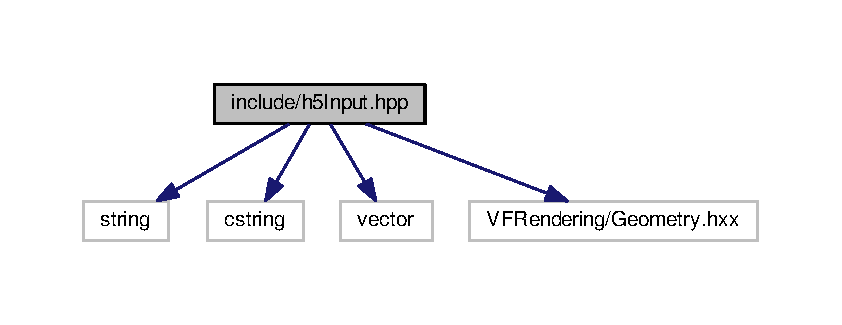
\includegraphics[width=350pt]{d9/d5d/h5Input_8hpp__incl}
\end{center}
\end{figure}
\subsection*{Namespaces}
\begin{DoxyCompactItemize}
\item 
 \hyperlink{namespaceh5Input}{h5\+Input}
\end{DoxyCompactItemize}
\subsection*{Functions}
\begin{DoxyCompactItemize}
\item 
void \hyperlink{namespaceh5Input_a7e2655a571daa8f456bc2a22eec1ef3d}{h5\+Input\+::get\+Field\+Temps} (std\+::string file\+Name, std\+::vector$<$ float $>$ \&Ts, std\+::vector$<$ float $>$ \&Hs)
\item 
void \hyperlink{namespaceh5Input_a4894a89d7f105d15e01f6c270d45b47a}{h5\+Input\+::get\+Spins} (std\+::string file\+Name, const int Tind, const int Hind, V\+F\+Rendering\+::\+Geometry \&geometry, std\+::vector$<$ glm\+::vec3 $>$ \&directions, std\+::vector$<$ double $>$ \&z\+\_\+pos)
\end{DoxyCompactItemize}

\hypertarget{renderOptions_8hpp}{}\section{include/render\+Options.hpp File Reference}
\label{renderOptions_8hpp}\index{include/render\+Options.\+hpp@{include/render\+Options.\+hpp}}
{\ttfamily \#include $<$Q\+Line\+Edit$>$}\\*
{\ttfamily \#include $<$Q\+Check\+Box$>$}\\*
{\ttfamily \#include $<$Q\+Push\+Button$>$}\\*
{\ttfamily \#include $<$vector$>$}\\*
Include dependency graph for render\+Options.\+hpp\+:
\nopagebreak
\begin{figure}[H]
\begin{center}
\leavevmode
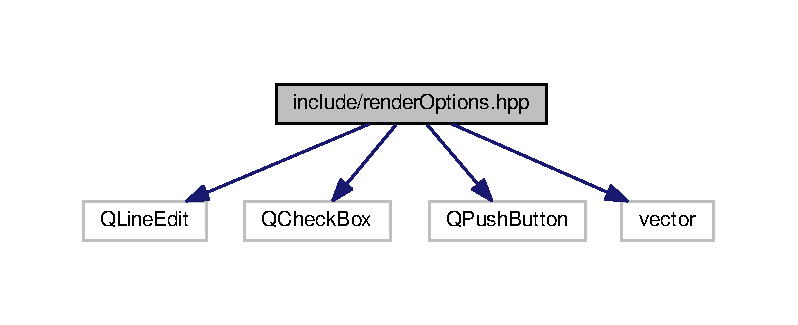
\includegraphics[width=350pt]{d7/d83/renderOptions_8hpp__incl}
\end{center}
\end{figure}
This graph shows which files directly or indirectly include this file\+:
\nopagebreak
\begin{figure}[H]
\begin{center}
\leavevmode
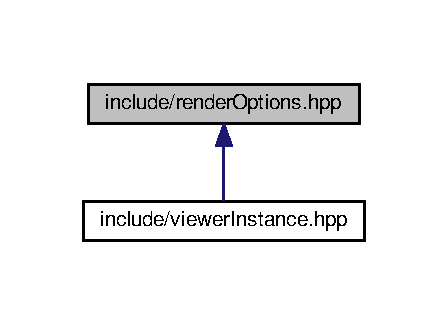
\includegraphics[width=215pt]{da/db0/renderOptions_8hpp__dep__incl}
\end{center}
\end{figure}
\subsection*{Classes}
\begin{DoxyCompactItemize}
\item 
class \hyperlink{classnMagWindows_1_1renderOptionsWindow}{n\+Mag\+Windows\+::render\+Options\+Window}
\end{DoxyCompactItemize}
\subsection*{Namespaces}
\begin{DoxyCompactItemize}
\item 
 \hyperlink{namespacenMagWindows}{n\+Mag\+Windows}
\end{DoxyCompactItemize}

\hypertarget{selectLatt_8hpp}{}\section{include/select\+Latt.hpp File Reference}
\label{selectLatt_8hpp}\index{include/select\+Latt.\+hpp@{include/select\+Latt.\+hpp}}
{\ttfamily \#include $<$string$>$}\\*
{\ttfamily \#include $<$vector$>$}\\*
{\ttfamily \#include $<$Q\+Push\+Button$>$}\\*
{\ttfamily \#include $<$Q\+Label$>$}\\*
{\ttfamily \#include $<$Q\+Slider$>$}\\*
Include dependency graph for select\+Latt.\+hpp\+:
\nopagebreak
\begin{figure}[H]
\begin{center}
\leavevmode
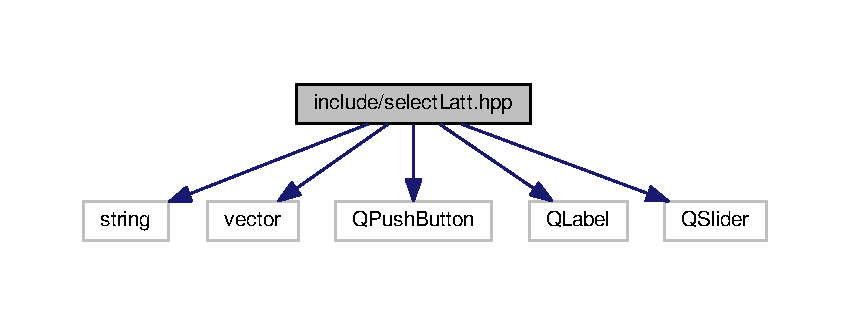
\includegraphics[width=350pt]{d0/d38/selectLatt_8hpp__incl}
\end{center}
\end{figure}
\subsection*{Classes}
\begin{DoxyCompactItemize}
\item 
class \hyperlink{classnMagWindows_1_1selectTHWindow}{n\+Mag\+Windows\+::select\+T\+H\+Window}
\end{DoxyCompactItemize}
\subsection*{Namespaces}
\begin{DoxyCompactItemize}
\item 
 \hyperlink{namespacenMagWindows}{n\+Mag\+Windows}
\end{DoxyCompactItemize}

\hypertarget{viewerInstance_8hpp}{}\section{include/viewer\+Instance.hpp File Reference}
\label{viewerInstance_8hpp}\index{include/viewer\+Instance.\+hpp@{include/viewer\+Instance.\+hpp}}
{\ttfamily \#include \char`\"{}render\+Options.\+hpp\char`\"{}}\\*
{\ttfamily \#include \char`\"{}viewer\+Window.\+hpp\char`\"{}}\\*
{\ttfamily \#include $<$string$>$}\\*
Include dependency graph for viewer\+Instance.\+hpp\+:\nopagebreak
\begin{figure}[H]
\begin{center}
\leavevmode
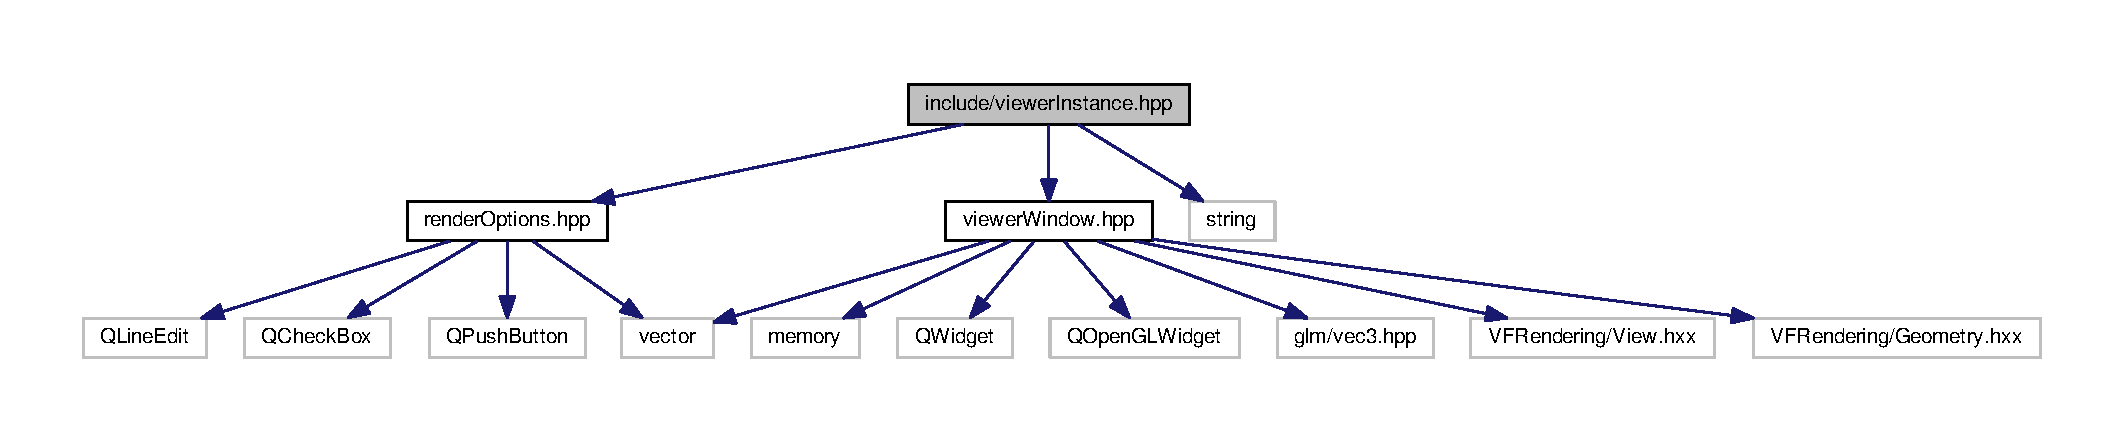
\includegraphics[width=350pt]{df/dd6/viewerInstance_8hpp__incl}
\end{center}
\end{figure}
\subsection*{Classes}
\begin{DoxyCompactItemize}
\item 
class \hyperlink{classnMagWindows_1_1viewerInstance}{n\+Mag\+Windows\+::viewer\+Instance}
\end{DoxyCompactItemize}
\subsection*{Namespaces}
\begin{DoxyCompactItemize}
\item 
 \hyperlink{namespacenMagWindows}{n\+Mag\+Windows}
\end{DoxyCompactItemize}

\hypertarget{viewerWindow_8hpp}{}\section{include/viewer\+Window.hpp File Reference}
\label{viewerWindow_8hpp}\index{include/viewer\+Window.\+hpp@{include/viewer\+Window.\+hpp}}
{\ttfamily \#include $<$memory$>$}\\*
{\ttfamily \#include $<$vector$>$}\\*
{\ttfamily \#include $<$Q\+Widget$>$}\\*
{\ttfamily \#include $<$Q\+Open\+G\+L\+Widget$>$}\\*
{\ttfamily \#include $<$glm/vec3.\+hpp$>$}\\*
{\ttfamily \#include $<$V\+F\+Rendering/\+View.\+hxx$>$}\\*
{\ttfamily \#include $<$V\+F\+Rendering/\+Geometry.\+hxx$>$}\\*
Include dependency graph for viewer\+Window.\+hpp\+:\nopagebreak
\begin{figure}[H]
\begin{center}
\leavevmode
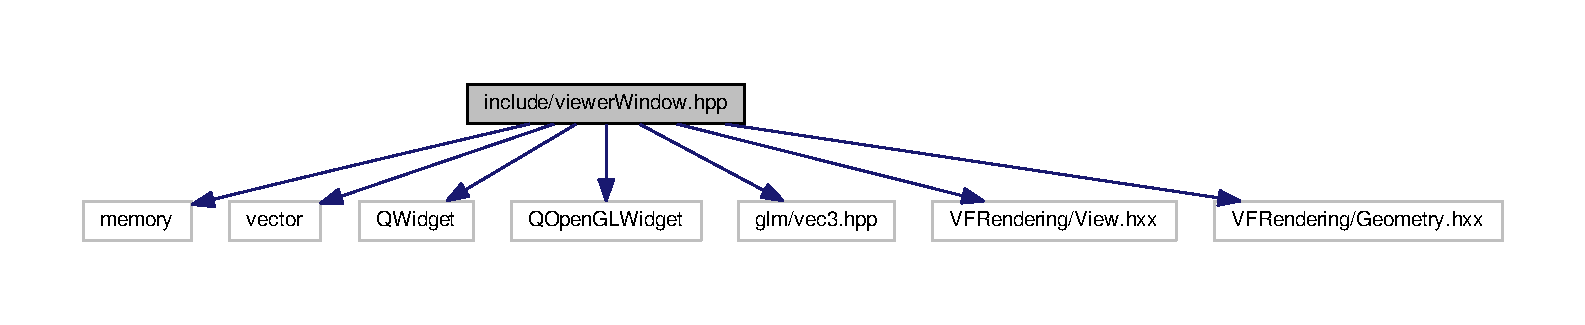
\includegraphics[width=350pt]{da/df8/viewerWindow_8hpp__incl}
\end{center}
\end{figure}
This graph shows which files directly or indirectly include this file\+:\nopagebreak
\begin{figure}[H]
\begin{center}
\leavevmode
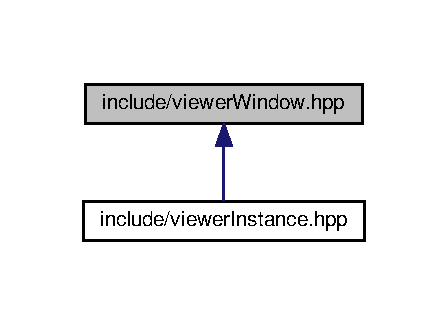
\includegraphics[width=215pt]{d3/dfb/viewerWindow_8hpp__dep__incl}
\end{center}
\end{figure}
\subsection*{Classes}
\begin{DoxyCompactItemize}
\item 
class \hyperlink{classnMagWindows_1_1viewerWindow}{n\+Mag\+Windows\+::viewer\+Window}
\end{DoxyCompactItemize}
\subsection*{Namespaces}
\begin{DoxyCompactItemize}
\item 
 \hyperlink{namespaceVFRendering}{V\+F\+Rendering}
\item 
 \hyperlink{namespacenMagWindows}{n\+Mag\+Windows}
\end{DoxyCompactItemize}

\hypertarget{README_8md}{}\section{R\+E\+A\+D\+M\+E.\+md File Reference}
\label{README_8md}\index{R\+E\+A\+D\+M\+E.\+md@{R\+E\+A\+D\+M\+E.\+md}}

%--- End generated contents ---

% Index
\backmatter
\newpage
\phantomsection
\clearemptydoublepage
\addcontentsline{toc}{chapter}{Index}
\printindex

\end{document}
